\chapter{Modeling 建模}
\intro{
	在每一个系统的探索中，存在第一性原理，这是一个最基本的命题或假设，不能被省略或删除，也不能被违反。
	
	\rightline{——亚里士多德}
	
	我倾向于从物理框架来研究事物。我们运用第一性原理，而不是类比思维去思考问题，是非常重要的
	
	\rightline{——埃隆·马斯克}
}
木一鲸家的程序员在他的文章中阐述了第一性原理。我觉得很对啊，第一性原理是物理世界最基本的原理。

所以这一章先记录一下第一性原理。
\section{第一性原理}
\subsection{ 第一性原理的内容}
第一性原理的核心思想是将问题分解为最基本、最不可分解的元素或原理。这些原理应当是不依赖于其他原理而能够自洽解释的。通过对这些基本原理的理解，可以构建对复杂系统的深刻理解。

\subsection{机器人学}
机器人最基本的元素是关节(joint)与连杆(link)，这就是机器人的第一性原理。

\begin{figure}[H]
\centering
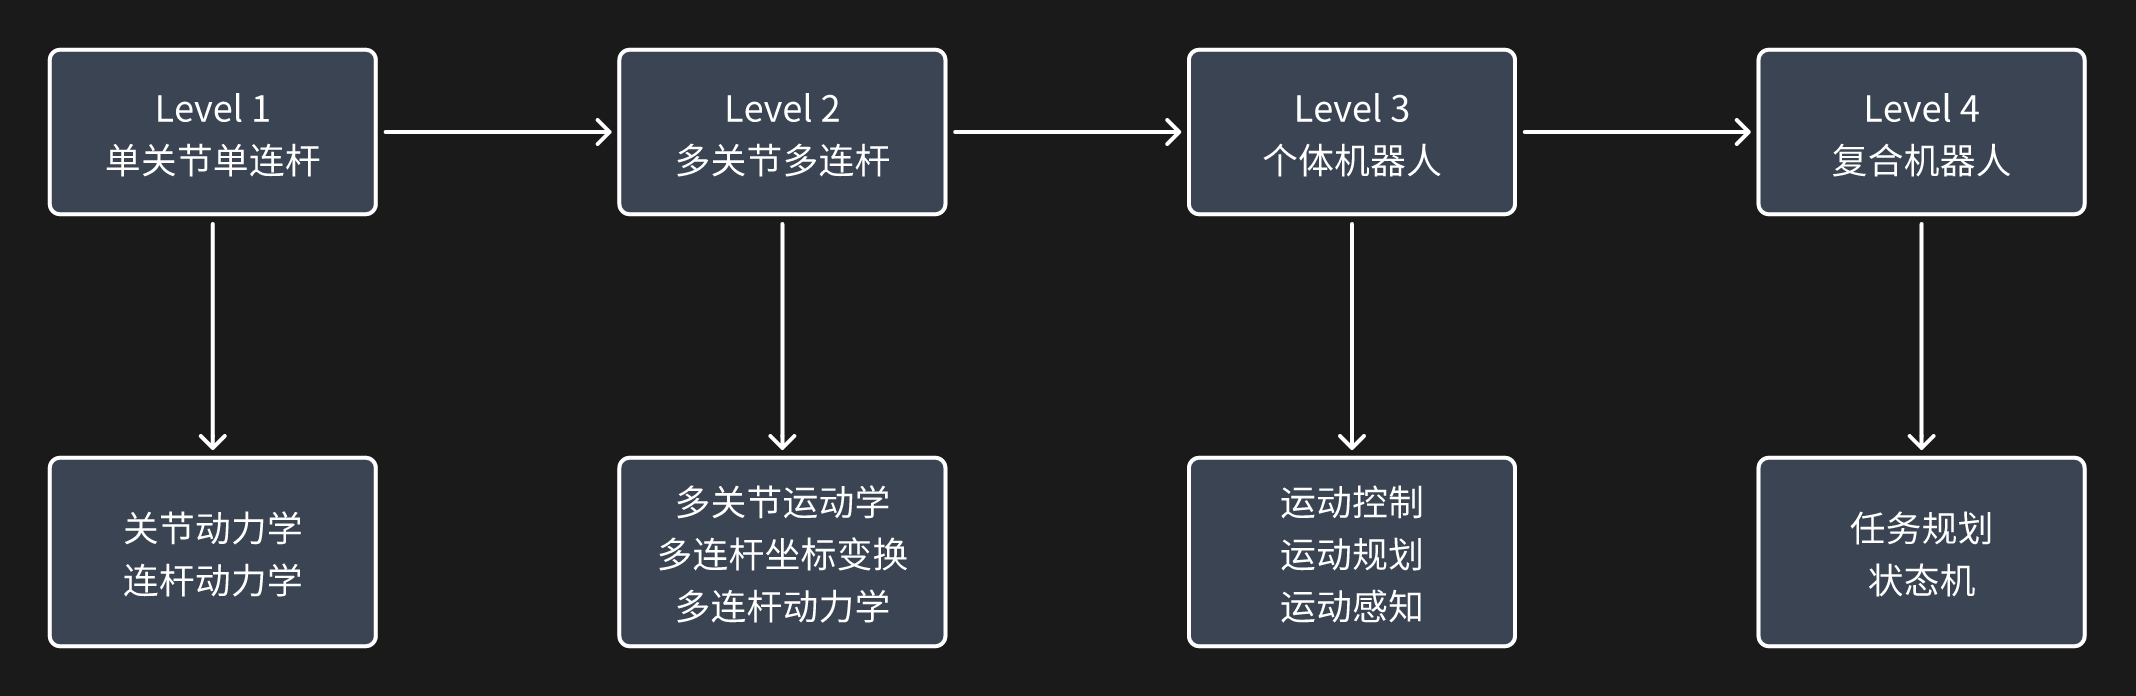
\includegraphics[width=0.6\linewidth]{Figure/第一性原理}
\caption{机器人的第一性原理}
\centering
\label{fig:1}
\end{figure}
\begin{itemize}
	\item[level 1：单关节-单连杆层面] 我们通常讨论关节动力学与连杆动力学
	\item[level 2: 多关节-多连杆层面] 我们通常考虑多关节运动学与连杆坐标变换，也会讨论多连杆动力学
	\item[level 3：个体机器人层面] 我们通常会讨论运动问题，即移动（足式与轮式）与操作问题。
	考虑到运动类型，我们又可以拆分成：
	
	固定基——机械臂
	
	浮动基——足式机器人与轮式机器人
	
	在操作问题中，我们通常考虑运动控制（关节力控，笛卡尔空间力控等），运动规划（轨迹规划，路径规划等）与运动感知（手眼协调等）
	
	在移动问题中，我们通常考虑运动控制（车辆动力学与控制等），运动规划（导航等）与运动感知（SLAM，三维重建等）
	\item[level 4：复合机器人层面] 我们通常会考虑任务规划，状态机等问题
\end{itemize}

\section{MJCF Mechanisms}
MJCF 使用多种模型创建机制，这些机制涵盖多个模型元素。为避免重复，本节仅对其进行一次详细描述。这些机制并不涉及计算章节之外的新仿真概念。它们的作用是简化 MJCF 模型的创建，并允许使用不同的数据格式，而无需手动转换为标准格式。

\subsection{Kinematics tree}
MJCF 文件的主要部分是由嵌套的 body 元素构成的 XML 树。顶层 body 元素比较特殊，称为 worldbody 。这种树状结构与 URDF 不同，URDF 先创建一系列链接，然后用连接符将它们连接起来，连接符指定子链接和父链接。在 MJCF 中，子 body 元素实际上是父 body 元素的子元素，这与 XML 的定义一致。
当在实体内部定义关节时，其功能并非连接父实体和子实体，而是创建它们之间的运动自由度。如果给定实体内部未定义任何关节，则该实体与其父实体焊接在一起。在 MJCF 中，一个实体可以包含多个关节，因此无需引入虚拟实体来创建复合关节。只需在同一个实体内定义构成所需复合关节的所有基本关节即可。例如，可以使用两个滑块和一个铰链来模拟在平面内运动的实体。
其他 MJCF 元素可以在由嵌套主体元素创建的树状结构中定义，特别是joint, geom, site, camera, light. 。当一个元素定义在某个物体内部时，它会被固定到该物体的局部坐标系中，并始终随该物体一起运动。引用多个物体或根本不引用任何物体的元素，则在运动学树之外的单独部分中定义。

\subsection{Default settings 默认设置}
MJCF 拥有完善的默认属性值设置机制。这使得我们能够拥有大量元素和属性，从而充分展现软件的丰富功能，同时还能编写简洁易读的模型文件。此外，该机制还允许用户在一个地方进行更改，并使其传播到整个模型。我们先来看一个例子。

\begin{lstlisting}
<mujoco>
<default class="main">
<geom rgba="1 0 0 1"/>
<default class="sub">
<geom rgba="0 1 0 1"/>
</default>
</default>

<worldbody>
<geom type="box"/>
<body childclass="sub">
<geom type="ellipsoid"/>
<geom type="sphere" rgba="0 0 1 1"/>
<geom type="cylinder" class="main"/>
</body>
</worldbody>
</mujoco>
\end{lstlisting}
这个示例实际上无法编译，因为缺少一些必要信息，但我们这里只关注几何图形的 rgba 值设置。上面创建的四个几何图形，根据默认设置机制，最终将具有以下 rgba 值：
\begin{table}[H]
	\centering
	\caption{}
	\begin{tabular}{ll}
		\textbf{geom type} & \textbf{geom rgba}  \\
		box                & 1 0 0 1             \\
		ellipsoid          & 0 1 0 1             \\
		sphere             & 0 0 1 1             \\
		cylinder~ ~        & 1 0 0 1            
	\end{tabular}
\end{table}

由于没有指定其他类，该立方体使用顶级默认类“main”来设置其未定义属性的值。该实体指定了子类“sub”，导致该实体的所有子对象（以及它们的子对象等等）都使用类“sub”，除非另有指定。因此，椭球体使用类“sub”。球体显式定义了 rgba，这会覆盖默认设置。圆柱体指定了默认类“main”，因此它使用“main”而不是“sub”，即使在包含该几何体的实体的子类属性中指定了后者。

\section{关节与连杆}
元素有四种类型：

\bigstar 